\documentclass{beamer}

\mode<presentation> {
\usecolortheme{seagull}

\setbeamertemplate{footline}[page number]}
\usepackage{graphicx} 
\usepackage{booktabs} 
\usepackage{url}
\usepackage{hyperref}

\AtBeginSection[]{
  \begin{frame}
  \vfill
  \centering
    \usebeamerfont{title}\Huge{\insertsectionhead\par}
  \vfill
  \end{frame}
}

%-------------------------------------------------------------------------

\title[TLKDCC Overview]{Linux Kernel Overview}
\author{Hans Holmberg}
\institute[LKTP]
{
Linux Kernel Teaching Project \\ 
\medskip
\textit{hans.holmberg@gmail.com}
}
\date{\today}
%------------------------------------------------------------------------
\begin{document}

\begin{frame}
\titlepage

\includegraphics{tux} 
\end{frame}

\begin{frame}
\frametitle{Overview}
\tableofcontents 
\end{frame}

%-----------------------------------------------------------------------
\section{What is Linux?} 

\begin{frame}
\frametitle{What is Linux?}
\begin{itemize}
	\item Linux is a Unix-like and mostly POSIX-compliant computer operating system (OS) assembled under the model of free and open-source software development and distribution. \footnote{Wikipedia on Linux \url{https://en.wikipedia.org/wiki/Linux}\\}
	\item The defining component of Linux is the Linux kernel, first released on September 17, 1991 by Linus Torvalds.
	\item Linux is sometimes referred to as GNU/Linux by the Free Software Foundation, as it relies of GNU code(such as the tool chain).
\end{itemize}
\end{frame}

\begin{frame}
\frametitle{Linux is everywhere}
25 years since it's creation, Linux now rules most of the planet's computer systems. \\
\begin{itemize}
	\item Servers
	\begin{itemize}
		\item First wide adoption of Linux
		\item Completely dominant
		\item Even Microsof is using Linux to run their cloud
	\end{itemize}
	\item Embedded 
	\begin{itemize}
		\item Phones: 1.3 Billion phones shipped with Android/Linux in 2015
		\item Runs lots and lots of other types of small devices(IOT/..)
	\end{itemize}
	\item Desktops - The exception, but any year now. 
\end{itemize}

\end{frame}

%-----------------------------------------------------------------------
\section{The kernel as part of the system}

\begin{frame}
\frametitle{The kernel piece in the puzzle}
The kernel's role in the system: \\
\begin{itemize}
	\item Hardware abstraction
	\item Provide services(IPC, networking, ..)
	\item Resource management(Memory, cpu time)
	\item Security
\end{itemize}
\end{frame}

\begin{frame}
\frametitle{The kernel ABI}
\begin{itemize}
	\item The Linux ABI is the kernel–user space API, which allows programs in user space to access system resources and services of the Linux kernel. It is composed out of the System Call Interface of the Linux kernel and the subroutines in the GNU C Library (glibc). which are resonably compatible with POSIX. 
The ABI can also be considered to include the interfaces provided in the virtual file system. 

	\item The Linux ABI must be backward compatible and must not break; this stability guarantees the portability of not only source code, but also pre-compiled programs. 
\end{itemize}
\end{frame}

\begin{frame}
\frametitle{The kernel ABI}
\begin{center}
	\includegraphics[width=0.8\textwidth]{kernel}
\end{center}
\end{frame}

\begin{frame}
\frametitle{Pitfalls}
\begin{itemize}
	\item Kernel headers (kernel *.h-files needed by user space)
User space and the kernel must have the same definition of structures passed over to the other side.\\
	\item 32 vs 64 bit - The kernel might be running in 64 bit while user space is 32 bit
Pointer problems and different definitions of long, be careful!
\end{itemize}
\end{frame}

%-----------------------------------------------------------------------
\section{Everything is a file}

\begin{frame}
\frametitle{"Everything" is a file in Linux}
\begin{itemize}
	\item "Everything is a file" describes one of the defining features of Unix, and its derivatives.

	\item Linux uses the file system abstraction to provide access to hardware,configuration and debug information by exposing files that can be read and written.
	\item Note that these special files are only exposed in file system name space - the files can be accessed like normal files but are not actually stored on any media.
\end{itemize}
\end{frame}

\begin{frame}
\frametitle{The Linux filesystem}
\textbf{sys}  : a means to export kernel data structures, their attributes, and the 
linkages between them to userspace \\
\textbf{configfs} : configuration of kernel objects from user space \\
\textbf{dev} : contains the special device files for all the devices \\
\textbf{proc} : more information to userspace (cmdline, version, devicetree) \\
\textbf{debugfs} : kernel to userspace debug information \\
\end{frame}

\begin{frame}
\frametitle{Examples}
\begin{itemize}
	\item /proc/version
	\item /proc/cmdline
	\item /sys/bus/mmc/devices/
\end{itemize}
\end{frame}

%-----------------------------------------------------------------------
\section{The kernel source code}

\begin{frame}
\frametitle{Upstream}

There are several different kernels being maintained and released from the upstream community at kernel.org\footnote{The Linux Kernel Archives \url{https://www.kernel.org}\\}.

\begin{itemize}
	\item Mainline (i.e 4.9-rc2)
	\begin{itemize}
		\item Maintained by Linus Torvalds, dictator
		\item Master tree, all new code is merged here
	\end{itemize}
	\item Stable and longterm: (i.e 4.4.30, 3.10.105)
	\begin{itemize}
		\item Maintained by Greg K-H and others
		\item Bugfixes(i.e. security flaws) and trivial support for new devices
	\end{itemize}
	\item Next 
	\begin{itemize}	
		\item Maintained by Stephen Rothwell
		\item Staging ground for new code from the maintainers
	\end{itemize}
\end{itemize}
\end{frame}

\begin{frame}
\frametitle{Source code anatomy overview}
\begin{itemize}
	\item \textbf{kernel} : core kernel code (i.e kernel initialization) \\
	\item \textbf{arch} : architecture specific code(i.e x86, arm, arm64, cris) \\
	\item \textbf{drivers} : device trivers (i.e, keyboards, mmc, ..) \\
	\item \textbf{documentation} : kernel documentation \\
	\item \textbf{scripts} : kernel utilities i.e(checkpatch, cleanpatch) \\
\end{itemize}

A really nice, cross-referenced web interface for accessing different version of the source code is prprovided by Free Electrons\footnote{LXR: \url{http://lxr.free-electrons.com/source/kernel/}\\}.
\end{frame}

\begin{frame}
\frametitle{Finding documentation}
\begin{itemize}
	\item Look in documentation/
	\item Read the code!
	\item Use the git history
	\item Google!
\end{itemize}
\end{frame}

\begin{frame}
\frametitle{Essential tools}
\textbf{git}
\begin{itemize}
	\item \textbf{clone} : clone(duplicate) a repository \\
	\item \textbf{checkout} : checkout a specific version\\
	\item \textbf{diff} : compare two revisions\\
	\item \textbf{log} : show commit history\\
	\item \textbf{blame} : figure out which commit changed a particular line\\
	\item \textbf{grep} : like normal grep, but faster in a git repo \\ 
\end{itemize}
\textbf{gitk} : graphical tool for browsing the history
\end{frame}

%-----------------------------------------------------------------------
\section{Building the kernel}

\begin{frame}
\frametitle{Kernel configuration}
Before building the kernel you need to configure it for your target system.
The .config file contains:
\begin{itemize}
	\item Configuration options
	\item Debug enablement
	\item Which drivers to build
\end{itemize}
\end{frame}

\begin{frame}[fragile]
\frametitle{.config example - Raspberry pi}
\begin{semiverbatim}
#
# Automatically generated file; DO NOT EDIT.
# Linux/arm 4.9.0-rc3 Kernel Configuration
#
CONFIG_ARM=y
CONFIG_ARM_HAS_SG_CHAIN=y
CONFIG_MIGHT_HAVE_PCI=y
CONFIG_SYS_SUPPORTS_APM_EMULATION=y
CONFIG_HAVE_PROC_CPU=y
CONFIG_STACKTRACE_SUPPORT=y
CONFIG_LOCKDEP_SUPPORT=y
CONFIG_TRACE_IRQFLAGS_SUPPORT=y
... and another 5732 lines
\end{semiverbatim}
\end{frame}

\begin{frame}
\frametitle{menuconfig}
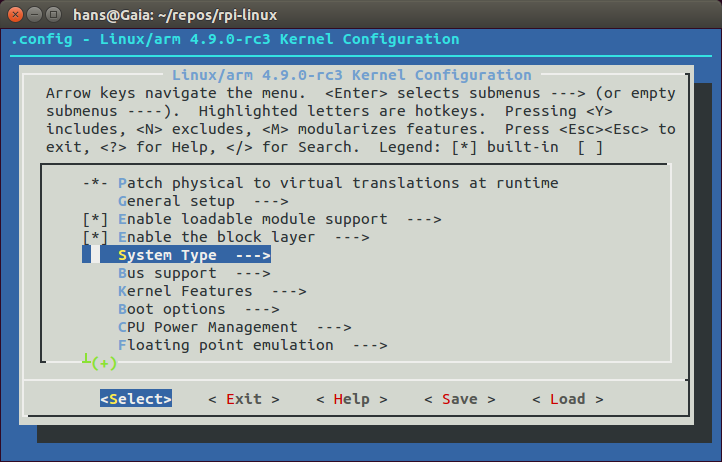
\includegraphics[width=\textwidth]{menuconfig.png}
\end{frame}

\begin{frame}[fragile]
\frametitle{Sample build flow, Raspberry pi}
\begin{semiverbatim}
\item make ARCH=arm bcm2835_defconfig
\item make ARCH=arm CROSS_COMPILE=arm-linux-gnueabihf- zImage
\item make ARCH=arm CROSS_COMPILE=arm-linux-gnueabihf- modules
\item make ARCH=arm CROSS_COMPILE=arm-linux-gnueabihf- dtbs
\item make modules_install INSTALL_MOD_PATH=/mnt/rpi-root
\item cp arch/arm/boot/zImage /mnt/rpi-root/boot
\item cp arch/arm/boot/dts/*.dtb /mnt/rpi-root/boot
\end{semiverbatim}
\end{frame}

%-----------------------------------------------------------------------
\begin{frame}
\Huge{\centerline{Thanks!}}
\end{frame}

\end{document} 
